\documentclass[journal,12pt,onecolumn]{IEEEtran}
\usepackage[utf8]{inputenc}   % Codificación de entrada
\usepackage[T1]{fontenc}      % Codificación de fuente
\usepackage[spanish,es-tabla]{babel}   % Idioma español
\usepackage{lmodern}          % Fuente moderna
\usepackage{amsmath, amssymb} % Matemáticas y símbolos
\usepackage{graphicx} 		  % Gráficos e imágenes
\graphicspath{{img/}{tablas/}{portada/}}  % Las imágenes se buscarán en la carpeta "img"
\usepackage{longtable}      % Para tablas que se extienden en varias páginas
\usepackage{tabularx}	% Tablas avanzadas
\usepackage{threeparttable}
\usepackage{hyperref}	% Hipervínculos
\usepackage{float} % va a servir para los espacios entre fotos supuestamente

%-------------------------------------------
% Otros paquetes útiles (personaliza según tus necesidades)
%-------------------------------------------
\usepackage{caption}
\usepackage{subcaption}
\usepackage{xcolor}
\usepackage{setspace}

%-------------------------------------------
% Comandos personalizados
\renewcommand{\listtablename}{Índice de tablas}
\renewcommand{\appendixname}{Anexos}
\definecolor{colorreferences}{RGB}{48,134,3}

% Metadatos del PDF
\hypersetup{
	unicode=true,
	hidelinks,
	colorlinks=true,       % false: boxed links; true: colored links
	linkcolor=black,          % color of internal links (change box color with linkbordercolor)
	citecolor=colorreferences,        % color of links to bibliography
	filecolor=magenta,      % color of file links
	urlcolor=blue,           % color of external links
	linkbordercolor={0 0 0}
}
%-------------------------------------------
% Inicio del documento
%-------------------------------------------
\begin{document}

% Aquí se encuentra el archivo con la portada
\begin{titlepage}
	\centering
	%-------------------------------------------
	% Logos en una tabla: izquierda, centro y derecha
	\begin{tabular}{@{}p{0.3\textwidth} p{0.3\textwidth} p{0.3\textwidth}@{}}
		
\includegraphics[height=2cm]{tecnm} & 
		\centering 
\includegraphics[height=1.5cm]{SEP} & 
		\raggedleft 
\includegraphics[height=2cm]{ith.jpg} \\
	\end{tabular}
	
	\vspace{2em}
	
	\noindent
	%-------------------------------------------
	%	Información institucional y académica (esquina superior izquierda)
	\begin{minipage}[t]{0.48\textwidth}
		\raggedright
		\small \textbf{%
			Instituto Tecnológico de Hermosillo\\
			Materia: Robótica\\
			Profesor: Medina Gil Lamadrid, Jesús Iván%
		}
	\end{minipage}%
	\hfill
	%	fecha actual (esquina superior derecha), en letras pequeñas y en negrita.
	\begin{minipage}[t]{0.48\textwidth}
		\raggedleft
		\small \textbf{\today}
	\end{minipage}
	
	\vspace{2em}
	
	%-----------------------------------------
	% Unidad y Título de la tarea en letras grandes y en negrita
	{\large \textbf{Unidad 1: Morfología del robot}}\\
	{\Huge \textbf{Tipos de Sensores}}
		
	\vspace{1em}
	
	%---------------------------------------
	% Tabla con la información del equipo
	%---------------------------------------
	% Encabezado del equipo
	\begin{center}
		{\Large \textbf{Equipo 2}}
	\end{center}
	
	\vspace{1em}
	
	% Tabla de integrantes:
	% Cada fila contiene: foto (columna izquierda) y datos del integrante (columna derecha)
	\begin{center}
		\begin{tabular}{c c}
			\begin{tabular}{c}
				
\includegraphics[height=3cm]{Cedano.jpeg} \\
				\textbf{Cedano Mendoza},\\ Carlos Francisco \\ \texttt{L21330552@hermosillo.tecnm.mx} \\ Teléfono: 6624686707
			\end{tabular} &
			\begin{tabular}{c}
				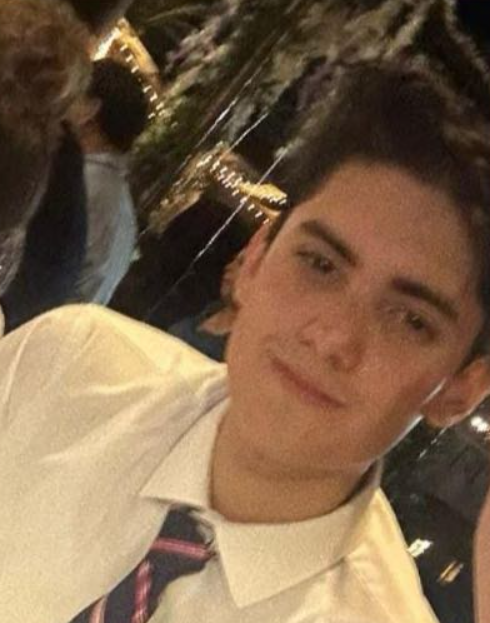
\includegraphics[height=3cm]{Martinez.png} \\
				\textbf{Martinez Navarro,}\\ Sebastian \\ \texttt{L2133} \\ Teléfono: 6621053764
			\end{tabular} \\ \vspace{2em}
			\begin{tabular}{c}
				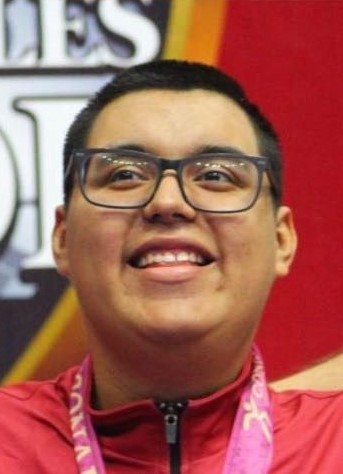
\includegraphics[height=3cm]{Ocampo.jpeg} \\
				\textbf{Ocampo Ramos,}\\ Addiel Adrián \\ \texttt{L20330895@hermosillo.tecnm.mx} \\ Teléfono: 6623501716
			\end{tabular} &
			\begin{tabular}{c}
				\includegraphics[height=3cm]{Pérez.jpeg} \\
				\textbf{Pérez Estupiñán,}\\ Ana Claudia \\ \texttt{L21330669@hermosillo.tecnm.mx} \\ Teléfono: 6624281154
			\end{tabular}
		\end{tabular}
	\end{center}

\end{titlepage}

%	Es innecesario poner el índice porque ya aparece en los marcadores del PDF
%\tableofcontents

% Ejemplo de inclusión de una sección (por ejemplo, "introduccion.tex" debe estar en la carpeta "secciones" y se recomienda no usar carácteres especiales (tilde) o espacios)


 \section{Sensores}
	Los sensores son dispositivos que permiten a los robots percibir su entorno y obtener información sobre su posición, movimiento, temperatura, proximidad, presión, entre otros aspectos. Estos sensores convierten datos físicos en señales eléctricas que el robot puede procesar para tomar decisiones o realizar tareas.

Se clasifican en:

	\subsection{Sensores Internos}
		\begin{enumerate}
			\item \textbf{Posición}
			
			Los sensores de posición miden la posición de cada articulación, es decir, el ángulo de articulación de un robot. A partir de dichos ángulos puede encontrarse la configuración del ejecutor final, y ubicar su posición y orientación por medio de la cinemática directa.\cite{saha2010robotics}\\
			
			
			\begin{enumerate}
				\item Lineal y rotativo
				\begin{enumerate}
					\item \textbf {Éncoders}
					 
			Es un dispositivo óptico digital que convierte el movimiento en una secuencia de pulsos digitales. Mediante el conteo de un solo bit o la decodificación de un conjunto de bits, los pulsos pueden convertirse en medidas relativas o absolutas. De este modo, los encóders son de tipo incremental o absoluto. Además, cada tipo puede ser lineal y rotatorio a su vez.\cite{saha2010robotics}\\
			
			\begin{enumerate}
				\item \underline{Éncoder lineal incremental:} \\
				Tiene una
				escala transparente con una retícula opaca. El tamaño del espesor de las líneas de la retícula y el del espacio entre ellas son iguales. De un lado, la escala se equipa con una fuente de luz y un lente de condensador. Del otro, hay celdas sensibles a la luz. La resistencia de las celdas (fotodiodos) disminuye cada vez que reciben un rayo de luz. De este modo, se genera un pulso cada vez que un rayo de luz es atravesado por la línea opaca. Este pulso se introduce en el controlador que actualiza a un contador \cite{saha2010robotics}.
				\\
		\begin{figure}[h]
	\centering
	\subfloat[Éncoder lineal incremental]{%
		\includegraphics[width=0.3\textwidth]{Velocidadsensoresdeposición.jpg}%
		\label{fig:Encoder_lineal_incremental}
		\cite{}
	}
	\hfill
\end{figure}				
\\
\\
\\
				\item \underline{Éncoder lineal absoluto:} \\
				En principio, se parece al encóder lineal incremental.  La diferencia es que da un valor absoluto de la distancia recorrida en cualquier momento. Así,
				las posibilidades de perder los pulsos a altas velocidades son menores. La salida es digital
				en este caso. La escala se marca con una secuencia de tiras opacas y transparentes. Si el bloque opaco que aparece en la escala de la ilustración (b)  representa 1 (uno) y el bloque transparente 0 (cero), entonces la columna de la extrema izquierda mostrará un número binario como 00000, es decir, un valor decimal de 0, y la columna siguiente mostrará un número binario 00001, es decir, una valor decimal de 1.\cite{saha2010robotics}
				
				\begin{figure}[h]
					\centering
					\subfloat[Perro]{%
						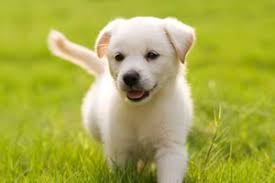
\includegraphics[width=0.4\textwidth]{perro.jpg}%
						\label{fig:perro}
					}
					\hfill
					\subfloat[Gato]{%
						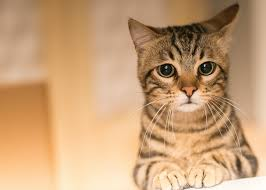
\includegraphics[width=0.4\textwidth]{gato.jpg}%
						\label{fig:gato}
					}
					\caption{Imagen de encoder lineal absoluto}
					\label{fig:mascotas}
				\end{figure}
				
				\item \underline{Éncoder rotativo lineal:} \\
				Se parece al encóder incremental lineal, con la diferencia
				de que las retículas se encuentran en este caso en un disco. El valor común del espesor de los espacios transparentes es igual a 20 micrones. Hay dos conjuntos de líneas de retículas en diferentes círculos que detectan el sentido de rotación, lo que permite mejorar la precisión del sensor. Hay otro círculo que sólo contiene una marca de retícula. Éste se usa para la medición del número
				de revoluciones completadas.\cite{saha2010robotics}
				\\
		\begin{figure}[h]
	\centering
	\subfloat[Éncoder lineal incremental]{%
		\includegraphics[width=0.3\textwidth]{Velocidadsensoresdeposición.jpg}%
		\label{fig:Encoder_lineal_incremental}
		\cite{}
	}
	\hfill
\end{figure}				
\\
\\
\\
\\
\\
\\

				\item \underline{Éncoder rotativo absoluto:} \\
				El disco se divide en un número de tiras circulares, y cada tira tiene segmentos de arco definidos, como se muestra en la figura. Este sensor proporciona directamente la salida digital (absoluta). El encóder se monta directamente sobre el eje del motor o con algún engranaje para aumentar la precisión de medición. Con el fin de evitar ruidos en este encóder, a veces se usa una escala gris. Un código gris, a diferencia de los códigos binarios, permite que sólo uno de los bits binarios en una secuencia de código cambie entre líneas radiales. También impide que se confundan los cambios en la salida binaria del encóder absoluto cuando el encóder oscila entre puntos. \cite {saha2010robotics}
				\\
				\begin{figure}[h]
					\centering
					\subfloat[Perro]{%
						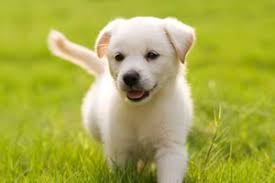
\includegraphics[width=0.4\textwidth]{perro.jpg}%
						\label{fig:perro}
					}
					\hfill
					\subfloat[Gato]{%
						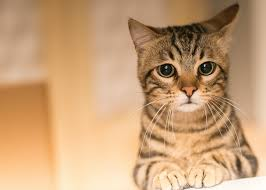
\includegraphics[width=0.4\textwidth]{gato.jpg}%
						\label{fig:gato}
					}
					\caption{Imagen de encoder rotativo absoluto}
					\label{fig:mascotas}
				\end{figure}
			\end{enumerate}
		
					\item \textbf{Potenciómetro}
					 
					Es un dispositivo de resistencia variable que expresa desplazamientos lineales o angulares en términos de voltaje, tal como se muestra en las figuras a) y b), respectivamente. Consiste en una clavija deslizante que hace contacto con un elemento resistivo; conforme se mueve este punto de contacto, la resistencia entre el contacto deslizante y las conexiones de los extremos del dispositivo cambia en proporción al desplazamiento, x y  para potenciómetros lineales
					y angulares, respectivamente. \cite{saha2010robotics}
					
				\begin{figure}[h]
					\centering
					\subfloat[Perro]{%
						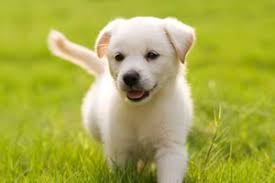
\includegraphics[width=0.4\textwidth]{perro.jpg}%
						\label{fig:perro}
					}
					\hfill
					\subfloat[Gato]{%
						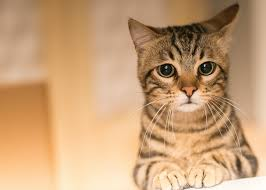
\includegraphics[width=0.4\textwidth]{gato.jpg}%
						\label{fig:gato}
					}
					\caption{Imagen de potenciometro}
					\label{fig:mascotas}
				\end{figure}


			\item \textbf{LVDT}
			\item \textbf{Resólver}
				\end{enumerate}
			\end{enumerate}
			
			\item \textbf{Velocidad}
			
            Los sensores de velocidad realizan la medición tomando medidas de posición consecutivas a intervalos de tiempo constante, calculando la razón de cambio respecto al tiempo de los valores de posición, o lo determina en forma directa con base en diferentes principios.\cite{saha2010robotics}\\
           
			
			\begin{enumerate}
				\item Todos los sensores de posición:
				Básicamente todos los sensores de posición, cuando se utilizan con ciertos límites de tiempo, pueden dar la velocidad, por ejemplo, el número de pulsos proporcionados por un encóder de posición incremental dividido entre el tiempo consumido en hacerlo. Sin embargo, este método impone una carga computacional sobre el controlador, que podrá estar ocupado por algunas otras operaciones.\\
		
		\begin{figure}[!ht]
			\centering
			\subfloat[Sensores de posición]{%
				\includegraphics[width=0.3\textwidth]{Velocidadsensoresdeposición.jpg}%
				\label{fig:sensores}
				\cite{Sensordeposición}
			}
			\hfill
		\end{figure}
				
				\item Tacómetro: Estos sensores pueden encontrar directamente la velocidad en cualquier momento y sin mucha carga computacional. Éstos miden la velocidad de rotación de un elemento. Hay varios tipos de tacómetros en uso, pero un diseño sencillo se basa en la regla de Fleming, que declara que “el voltaje producido es proporcional al índice del acoplamiento inductivo”. Aquí un conductor (básicamente una bobina) se sujeta al elemento rotativo que gira en un campo magnético (estator). Conforme incrementa la velocidad del eje, el voltaje producido en las terminales de las bobinas también aumenta.\cite{saha2010robotics}\\
				
				\begin{figure}[h]
					\centering
					\subfloat[Tacómetro]{%
						\includegraphics[width=0.3\textwidth]{Tacómetro.jpg}%
						\label{fig:Tacómetro}
						\cite{Tacómetro}
					}
					\hfill
				\end{figure}
				
				\item Sensor de efecto Hall: Es un dispositivo que se utiliza para medir la magnitud de un campo magnético. Su función se basa en el fenómeno físico conocido como el efecto Hall, por el cual se genera una diferencia de potencial eléctrico, o voltaje Hall, a través de un material conductor cuando este se encuentra dentro de un campo magnético y se le hace pasar una corriente eléctrica. Este fenómeno fue descubierto en 1879 por el físico estadounidense Edwin Hall.\cite{Hall} \\
				
			\begin{figure}[h]
				\centering
				\subfloat[EfectoHall]{%
					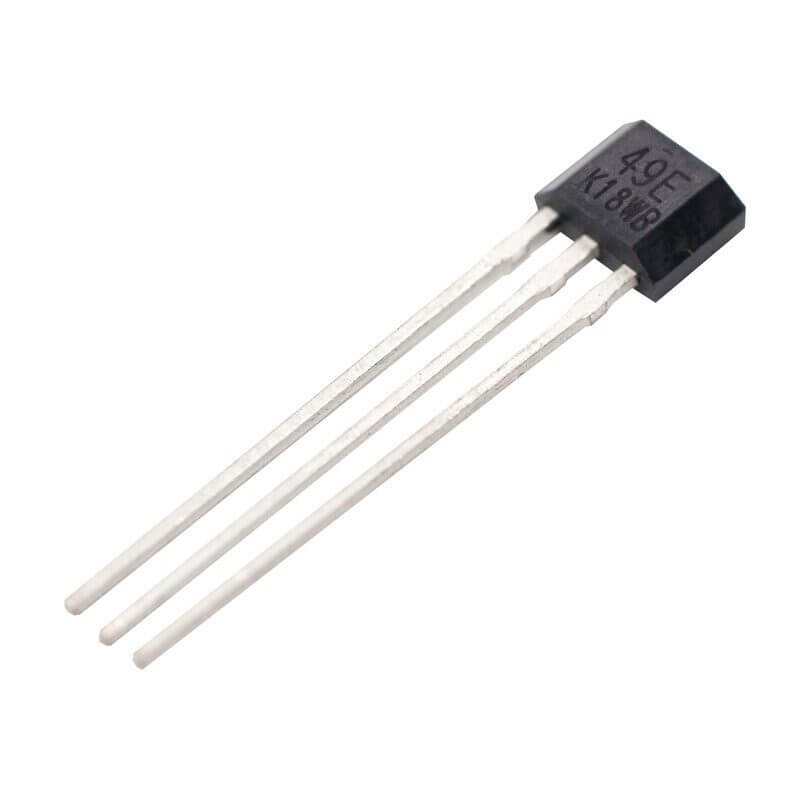
\includegraphics[width=0.25\textwidth]{Hall.jpg}%
					\label{fig:Hall}
					\cite{EfectoHall}
				}
				\hfill
			\end{figure}
			
			\end{enumerate}
			
			\item \textbf{Aceleración}
			
			Los Sensores de aceleración son dispositivos que mide la aceleración experimentada por un objeto en movimiento. Funciona detectando cambios en la velocidad del objeto en una dirección particular. Cuando un objeto acelera, cambia su velocidad en esa dirección, y el sensor de aceleración registra este cambio. \cite{Aceleración} \\
			
			\begin{enumerate}
				\item Todos los sensores de fuerza: De manera parecida a las mediciones de velocidad que se dan a partir de la información de los sensores de posición, pueden encontrarse las aceleraciones como la razón de cambio respecto al tiempo de las velocidades obtenidas por los sensores de velocidad o calculado a partir de las informaciones de posición. Pero ésta no es una manera efi ciente para calcular la aceleración, puesto que impondrá una carga de trabajo pesada sobre la computadora, lo que puede reducir la velocidad de operación del sistema. Otra forma de medir la aceleración es calculando la fuerza que resulta de multiplicar masa por aceleración. \cite{saha2010robotics}\\
			\end{enumerate}
				\begin{figure}[h]Acelerac
				\centering
				\subfloat[Aceleración]{%
					\includegraphics[width=0.25\textwidth]{Aceleración.jpg}%
					\label{fig:Aceleración}
					\cite{ión}
				}
				\hfill
			\end{figure}
			
			\item \textbf{Fuerza}
			
			Una balanza de resorte es un ejemplo de un sensor de
			fuerza en donde se aplica una fuerza, por ejemplo, el peso, al platillo de balanza que causa un desplazamiento, es decir, el resorte se estira. El desplazamiento es entonces una medida de la fuerza. Existen otros tipos de sensores de fuerza, por ejemplo, con base en galgas, utilizando el sensor de efecto Hall, etcétera. \cite{saha2010robotics}\\
			\begin{enumerate}
				\item Galgas extensométricas:
				
				\item Interruptores de límite:
				
				\item Interruptores piezoeléctricos:
				
			\end{enumerate}
		\end{enumerate}
		
	\subsection{Sensores Externos}
	 \begin{enumerate}
		\item \textbf{Tipo de contacto}
		\begin{enumerate}
			\item Interruptores de límite
			\item Interruptores neumáticos
			\item Sensores piezoeléctricos
			\item Transductores de presión
		\end{enumerate}
		\item \textbf{Tipo sin contacto}
		\begin{enumerate}
			\item Sensores de proximidad:  Es un dispositivo que detecta la presencia o ausencia de un objeto dentro de un rango específico sin necesidad de contacto físico. Este tipo de sensor es ampliamente utilizado en aplicaciones industriales y de automatización debido a su capacidad para operar en entornos donde el contacto directo podría ser problemático o dañino.\cite{Prox}\\ 
			\begin{figure}[h]
				\centering
				\subfloat[Sensor de proximidad]{%
					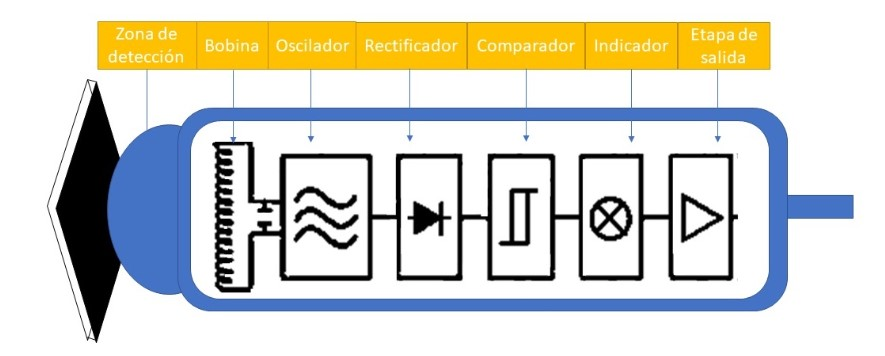
\includegraphics[width=0.20\textwidth]{Prox.jpg}%
					\label{fig:Sensor de proximidad}
					\cite{Prox}
				}
				\hfill
			\end{figure}
			\item Sensores de efecto Hall: Es un dispositivo que utiliza el efecto Hall para detectar campos magnéticos y convertir esta medición en una señal eléctrica. Este tipo de sensor es particularmente útil en aplicaciones donde se requiere la detección de la proximidad o la posición de objetos magnéticos sin necesidad de contacto físico.\cite{EHall}\\ 
			\begin{figure}[h]
				\centering
				\subfloat[Sensor de efecto Hall]{%
					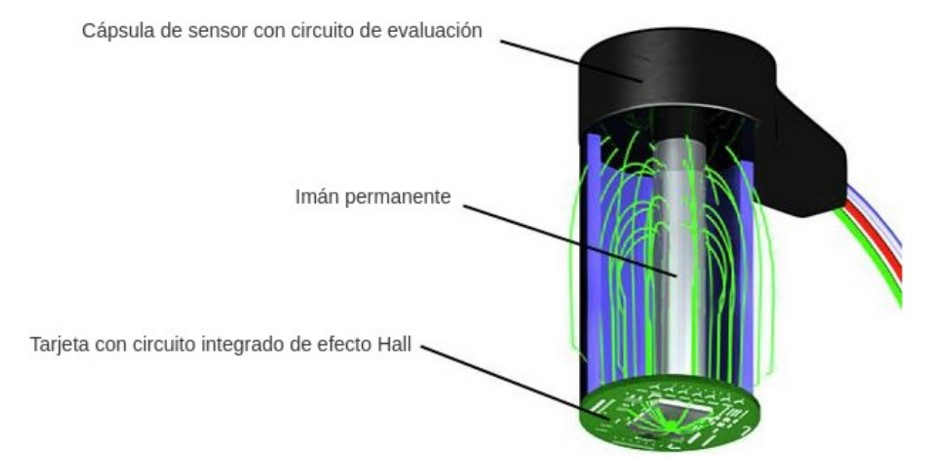
\includegraphics[width=0.20\textwidth]{SHall.jpg}%
					\label{fig:Sensor de efecto Hall}
					\cite{EHall}
				}
				\hfill
			\end{figure}
			\item Sensores de microondas: son dispositivos electrónicos que utilizan radiación de microondas para detectar movimiento, presencia o distancia sin necesidad de contacto físico. Estos sensores son especialmente útiles en aplicaciones donde la detección sin contacto es crucial, como en sistemas de seguridad, automatización industrial y control de tráfico.\cite{microo}\\ 
			\begin{figure}[h]
				\centering
				\subfloat[Sensores de microondas]{%
					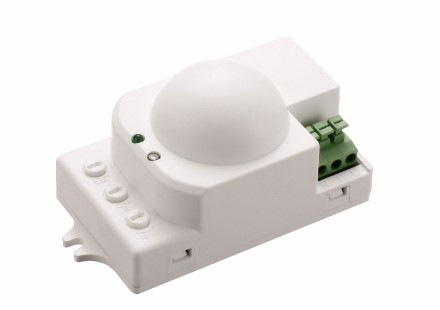
\includegraphics[width=0.20\textwidth]{Microoondas.jpg}%
					\label{fig:Sensores de microondas}
					\cite{microo}
				}
				\hfill
			\end{figure}
			\item Sensores ultrasónicos: Son dispositivos que utilizan ondas sonoras de alta frecuencia para medir distancias y detectar objetos sin contacto físico. Estos sensores son particularmente útiles en aplicaciones industriales y automatización, donde la precisión y la fiabilidad son esenciales.\cite{ultrason}\\ 
			\begin{figure}[h]
				\centering
				\subfloat[Sensores ultrasónicos]{%
					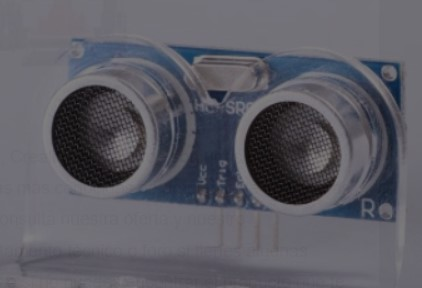
\includegraphics[width=0.20\textwidth]{Ultrasonico.jpg}%
					\label{fig:Sensores ultrasónicos}
					\cite{ultrason}
				}
				\hfill
			\end{figure}
			\item Sensores láser: Son dispositivos ópticos que utilizan un haz de luz láser para medir distancias, posiciones y detectar objetos sin contacto físico. Su capacidad para operar sin necesidad de tocar el objeto a medir los convierte en herramientas valiosas en diversas aplicaciones industriales y tecnológicas.\cite{Slaser}\\ 
			\begin{figure}[h]
				\centering
				\subfloat[Sensores láser]{%
					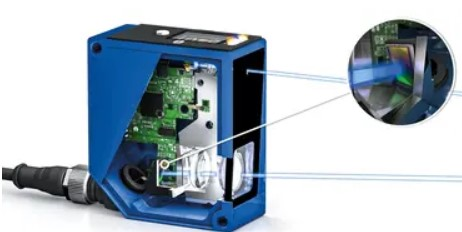
\includegraphics[width=0.15\textwidth]{SensorLaser.jpg}%
					\label{fig:Sensores láser}
					\cite{Slaser}
				}
				\hfill
			\end{figure}
			\item Sensores de visión: Son dispositivos que utilizan tecnología de imagen para detectar y analizar objetos sin necesidad de contacto físico. Estos sensores son parte integral de los sistemas de visión artificial y se emplean en diversas aplicaciones industriales, como inspección de calidad, control de procesos y automatización.\cite{Svision}\\ 
			\begin{figure}[h]
				\centering
				\subfloat[Sensores de visión]{%
					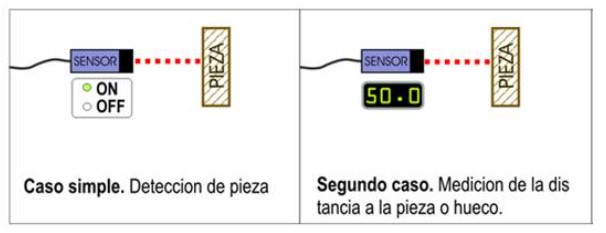
\includegraphics[width=0.20\textwidth]{SensorVision.jpg}%
					\label{fig:Sensores de visión}
					\cite{Svision}
				}
				\hfill
			\end{figure}
		\end{enumerate}
	\end{enumerate}

Para usar dos imágenes como en \autoref{fig:mascotas}, se utilizó \texttt{subfloat}.
% Dos imágenes de mascotas
\begin{figure}[h]
	\centering
	\subfloat[Perro]{%
		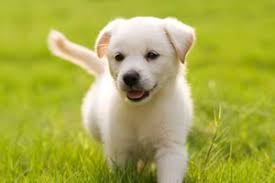
\includegraphics[width=0.4\textwidth]{perro.jpg}%
		\label{fig:perro}
	}
	\hfill
	\subfloat[Gato]{%
		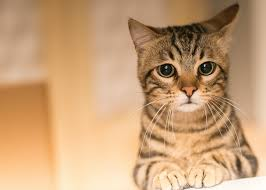
\includegraphics[width=0.4\textwidth]{gato.jpg}%
		\label{fig:gato}
	}
	\caption{Imagen de dos mascotas}
	\label{fig:mascotas}
\end{figure}
\section{Tablas}
Existen varias formas de crear tablas además de este entorno, como \texttt{array}, \texttt{longtable} y \texttt{tabularx}, que permiten manejar datos extensos de manera eficiente. También es posible convertirlas desde páginas, como en \href{https://tableconvert.com/es/excel-to-latex}{TableConvert}, que permite transformar datos de Excel a formato \LaTeX fácilmente.

A continuación, se presenta una tabla larga como ejemplo:

\newcounter{actividad} % Define un contador llamado "actividad"
\begin{longtable}{|c|p{10cm}|c|} % Define anchos específicos
	\caption{Ejemplo de Tabla Larga.} \label{tab:ejemplo_tabla} \\
	\hline
	\textbf{No.} & \textbf{Descripción} & \textbf{Estado} \\
	\hline
	\endfirsthead
	\multicolumn{3}{c}{{\tablename\ \thetable{} -- continuación}} \\
	\hline
	\textbf{No.} & \textbf{Descripción} & \textbf{Estado} \\
	\hline
	\endhead
	\hline \multicolumn{3}{r}{{Continúa en la siguiente página...}} \\
	\hline
	\endfoot
	\hline
	\endlastfoot
	% Contenido de la tabla
	1 & Lorem ipsum dolor sit amet, consectetur adipiscing elit. & Completado \\
	2 & Sed do eiusmod tempor incididunt ut labore et dolore magna aliqua. & En proceso \\
	3 & Ut enim ad minim veniam, quis nostrud exercitation ullamco laboris. & Pendiente \\
	4 & Duis aute irure dolor in reprehenderit in voluptate velit. & Pendiente \\
	5 & Excepteur sint occaecat cupidatat non proident. & Pendiente \\
	6 & Sunt in culpa qui officia deserunt mollit anim id est laborum. & Pendiente \\
	7 & Curabitur pretium tincidunt lacus, nulla gravida orci a odio. & Pendiente \\
	8 & Nullam varius, turpis et commodo pharetra. & Pendiente \\
	9 & Sed ac orci quis tortor imperdiet venenatis. & Pendiente \\
	10 & Duis eget orci sit amet orci dignissim rutrum. & Pendiente \\
	11 & Nam dui ligula, fringilla a, euismod sodales, sollicitudin vel, wisi. & Pendiente \\
	12 & Pellentesque habitant morbi tristique senectus et netus et malesuada. & Pendiente \\
	13 & Fusce convallis metus id felis luctus adipiscing. & Pendiente \\
	14 & Pellentesque dapibus hendrerit tortor. & Pendiente \\
	15 & Praesent egestas tristique nibh. & Pendiente \\
	16 & Curabitur a felis in nunc fringilla tristique. & Pendiente \\
	17 & Phasellus nec sem in justo pellentesque facilisis. & Pendiente \\
	18 & Etiam imperdiet imperdiet orci. & Pendiente \\
	19 & Vestibulum ante ipsum primis in faucibus orci luctus et ultrices. & Pendiente \\
	20 & Quisque id mi. Integer ante arcu, accumsan a, consectetuer eget, posuere ut, mauris. & Pendiente \\
\end{longtable}
\section{Ecuaciones}
Para realizar ecuaciones, se pueden ayudar mucho de ChatGPT (Como copiar una imagen y que lea la ecuación para dártela en formato \LaTeX) y de que MATLAB, word y algunas páginas te permiten copiar ecuaciones en formato \LaTeX. El modelo en espacio de estados de un robot de dos grados de libertad, el cual se puede ver en el Capítulo 5: Dinámica del Robot en \cite{barrientos2007fundamentos} se expresa como

\begin{equation}
	\label{eq:spaceStateRobot}
	\begin{bmatrix}
		\dot{q} \\
		\ddot{q}
	\end{bmatrix} =
	\begin{bmatrix}
		0 & I \\
		M^{-1}(-C - G)
	\end{bmatrix}
	\begin{bmatrix}
		q \\
		\dot{q}
	\end{bmatrix} +
	\begin{bmatrix}
		0 \\
		M^{-1} B
	\end{bmatrix} u,
\end{equation}
donde:
\begin{itemize}
	\item \( q \) es el vector de posiciones articulares del robot.
	\item \( \dot{q} \) y \( \ddot{q} \) son las velocidades y aceleraciones articulares.
	\item \( M \) es la matriz de inercia.
	\item \( C \) representa las fuerzas centrífugas y de Coriolis.
	\item \( G \) es el vector de fuerzas gravitacionales.
	\item \( B \) es la matriz de entrada de los torques.
	\item \( u \) es el vector de torques aplicados a las articulaciones.
\end{itemize}

Cabe destacar que en \eqref{eq:spaceStateRobot}, la ecuación se referencia después de haberla nombrado y forma parte de la oración, por lo que debe llevar puntos o comas. También al referenciar, debe de estar entre paréntesis con \texttt{eqref}.
\section{Conclusión}
En la elaboración de este reporte, se utilizó por primera vez el software LaTeX para la edición del documento y Sourcetree para la gestión del control de movimientos entre modificaciones de datos del documento por parte de los distintos miembros del equipo. A lo largo del proceso, se presentaron dificultades relacionadas con el uso de Sourcetree, especialmente en la ejecución de comandos como branches, commit, push y pull, lo que requirió una curva de aprendizaje adicional para comprender su funcionamiento y evitar conflictos en la sincronización de archivos.

A pesar de estos desafíos, la experiencia permitió familiarizarse con herramientas clave para la edición y gestión colaborativa de documentos, lo que resultará beneficioso en futuros proyectos. La combinación de LaTeX y Sourcetree demostró ser una opción robusta para la elaboración de reportes técnicos con un control de organización eficiente, aunque es recomendable seguir profundizando en su uso para optimizar los flujos de trabajo y minimizar errores.

Por otra parte, el conocimiento más importante obtenido de la investigación sobre los distintos tipos de sensores fue la comprensión de cómo cada tecnología responde a necesidades específicas en diversas industrias. Esta investigación permitió no solo identificar las aplicaciones clave de cada sensor, sino también comprender la importancia de la selección adecuada según el entorno y el tipo de medición requerida. La evolución de los sensores, junto con su integración con inteligencia artificial y procesamiento de datos, sigue impulsando innovaciones en automatización, control y análisis del entorno.









%-------------------------------------------
% Bibliografía
%-------------------------------------------
\bibliographystyle{IEEEtran}  % Estilo de bibliografía IEEE
% La bibliografía se tomará del archivo "fuentes.bib"
\bibliography{fuentes}
	
\end{document}
